\chapter{Технологическая часть}

В данном разделе будут представлены реализации алгоритма бинарного поиска в словаре и алгоритма определения соответствия введённого запроса распознаваемым вариантам. Также будут указаны обязательные требования к ПО, средства реализации алгоритмов, представлены интерфейс разработанного веб-сервиса и результаты проведённого тестирования программы.

\section{Требования к ПО}
Для программы выделен перечень требований:
\begin{itemize}
	\item программой предоставляется интерфейс в формате веб-сервиса с поисковой строкой;
	\item программой обрабатываются запросы, сформированный по указанным ниже требованиям;
	\item программой не воспринимаются запросы, не соответствующие требованиям, выводится сообщение об ошибке;
	\item программой производится аварийное завершение с текстом об ошибке при иных ошибках;
	\item программой выводится список удовлетворяющих запросу данных с иллюстрациями при валидном запросе.
\end{itemize}

\section{Требования к входному запросу}
Запрос может быть воспринят программой, как валидный, если он удовлетворяет следующим правилам:
\begin{itemize}
	\item «выведи», «дай», «показывай», «покажи», «какие», «выдай», «хочу», «найти», «найди» в качестве вводного слова, при этом само наличие вводного слова является необязательным в запросе;
	\item «кошка», «кот», «котёнок», «кошечка», «котик», «котёночек» и другие формы этих слов, приводимые при нормализации к указанной, при этом наличие подобного указания на тип объекта является обязательным;
	\item Указанные далее категории в начальной или иной форме слова; категории объединены в классы эквивалентности символом «-»: «лысый»-«не пушистый», «плешивый»-«не особо пушистый»-«не пушистый»-«не лысый», «волосатый»-«не особо пушистый»-«не пушистый»-«не очень пушистый»-«не лысый», «пушистый»-«не лысый»-«немного пушистый», «очень пушистый»-«не лысый»-«сильно пушистый», «невероятно пушистый»-«не лысый»;
	\item вводное слово обязано быть первым в запросе, если оно есть, порядок слова-объекта и слова-категории относительно друг друга может быть любым.
\end{itemize}

\section{Средства реализации}
Для реализации данной работы был выбран язык программирования Go \cite{item1}. Выбор обусловлен наличием в $Go$ библиотек для тестирования ПО, работы с $http$ протоколом \cite{item7}, а также необходимых для реализации поставленных цели и задач средств. В качестве среды разработки была выбрана $GoLand$ \cite{item3}. Для хранения данных о котах была создана база данных $cats$ с помощью СУБД $Postgres$ \cite{item10}.

\section{Реализация алгоритмов}
В листингах \ref{code:bin1}~--~\ref{code:rec3} представлены реализации алгоритма бинарного поиска в словаре и алгоритма определения соответствия введённого запроса распознаваемым вариантам. 

\begin{code}
\caption{Листинг функции реализации алгоритма бинарного поиска в словаре (начало)}
\label{code:bin1}
\begin{minted}{go}
func (d *Dictionary) BinarySearch(key int, isStart bool) int {
	last := len(*d) - 1
	if key > (*d)[last].Key {
		return last
	}
	if key < (*d)[0].Key {
		return 0
	}
	lo := 0
	hi := last
\end{minted}
\end{code}

\begin{code}
\caption{Листинг функции реализации алгоритма бинарного поиска в словаре (продолжение листинга \ref{code:bin1})}
\label{code:bin2}
\begin{minted}{go}
	for lo <= hi {
		m := (lo + hi) / 2
		if key > (*d)[m].Key {
			lo = m + 1
		} else if key < (*d)[m].Key {
			hi = m - 1
		} else {
			return m
		}
	}
	crossed := (*d)[lo].Key > (*d)[hi].Key
	if crossed == isStart {
		return lo
	}
	return hi
}
\end{minted}
\end{code}

\begin{code}
\caption{Листинг функции алгоритма определения соответствия введённого запроса распознаваемым вариантам (начало)}
\label{code:rec1}
\begin{minted}{go}
func IsCorrectQuery(tokens []string) (int, int, error) {
	start := 0

	for _, v := range Starters {
		if tokens[0] == v {
			start = 1
			break
		}
	}
	subquery := strings.Join(tokens[start:], " ")

	start = -1
	length := 0
\end{minted}
\end{code}

\begin{code}
\caption{Листинг функции алгоритма определения соответствия введённого запроса распознаваемым вариантам (продолжение листинга \ref{code:rec1})}
\label{code:rec2}
\begin{minted}{go}
	for i, v := range Objects {
		if strings.Contains(subquery, v) {
			if len(v) > length {
				length = len(v)
				start = i
			}
		}
	}

	if start == -1 {
		return -1, -1, errors.New("неверный объект запроса")
	} else {
		subquery = strings.Replace(subquery, Objects[start], "", 1)
		subquery = strings.TrimSpace(subquery)
	}
	
	start = -1
	end := -1
	
	for _, v := range Intervals {
		for _, e := range v.Names {
			if subquery == e {
				if start == -1 {
					start = v.Start
				}
				if v.End > end {
					end = v.End
				}
			}
		}
	}
\end{minted}
\end{code}

\newpage

\begin{code}
\caption{Листинг функции алгоритма определения соответствия введённого запроса распознаваемым вариантам (продолжение листинга \ref{code:rec2})}
\label{code:rec3}
\begin{minted}{go}
	if start == -1 || end == -1 {
		return -1, -1, errors.New("некорректный формат запроса")
	}

	return start, end, nil
}
\end{minted}
\end{code}

\section{Реализация структуры словаря}
В листинге \ref{code:str} представлена реализации структуры словаря.

\begin{code}
\caption{Листинг реализации структуры словаря}
\label{code:str}
\begin{minted}{go}
type Word struct {
	Key   int
	Value models.Cat
}

type Dictionary []Word
\end{minted}
\end{code}

\newpage

\section{Тестирование}
В таблице \ref{table:tests} представлены тесты запросов для поиска в словаре. Все тесты пройдены успешно.

\begin{table}[H]
  \caption{\label{table:tests} Тесты для поиска в словаре}
  \begin{center}
    \begin{tabular}{|c|c|c|}
      \hline
      № &  Запрос & Результат \\ \hline
      1 & найти плешивых котиков & \specialcell{Ориентальная\\Количество пушинок на квадратный см – 424!\\...} \\ \hline
      2 & дай пушистых котят & \specialcell{Нибелунг\\Количество пушинок на квадратный см – 8777!\\...} \\ \hline
      3 & невероятно пушистые кошечки & \specialcell{Сибирская\\Количество пушинок на квадратный см – 18005!\\...} \\ \hline
      4 & невероятно пушистые рыбки & \specialcell{Ошибка выполнения запроса:\\неверный объект запроса}  \\ \hline
      5 & покажи короче котов мне быстро & \specialcell{Ошибка выполнения запроса:\\ некорректный формат запроса}\\ \hline
    \end{tabular}
  \end{center}
\end{table}

\newpage

\section{Интерфейс веб-сервиса}
На рисунках \ref{img:int1}~--~\ref{img:int2} представлен интерфейс разработанного веб-сврвиса.

\begin{figure}[h!]
    \centering
    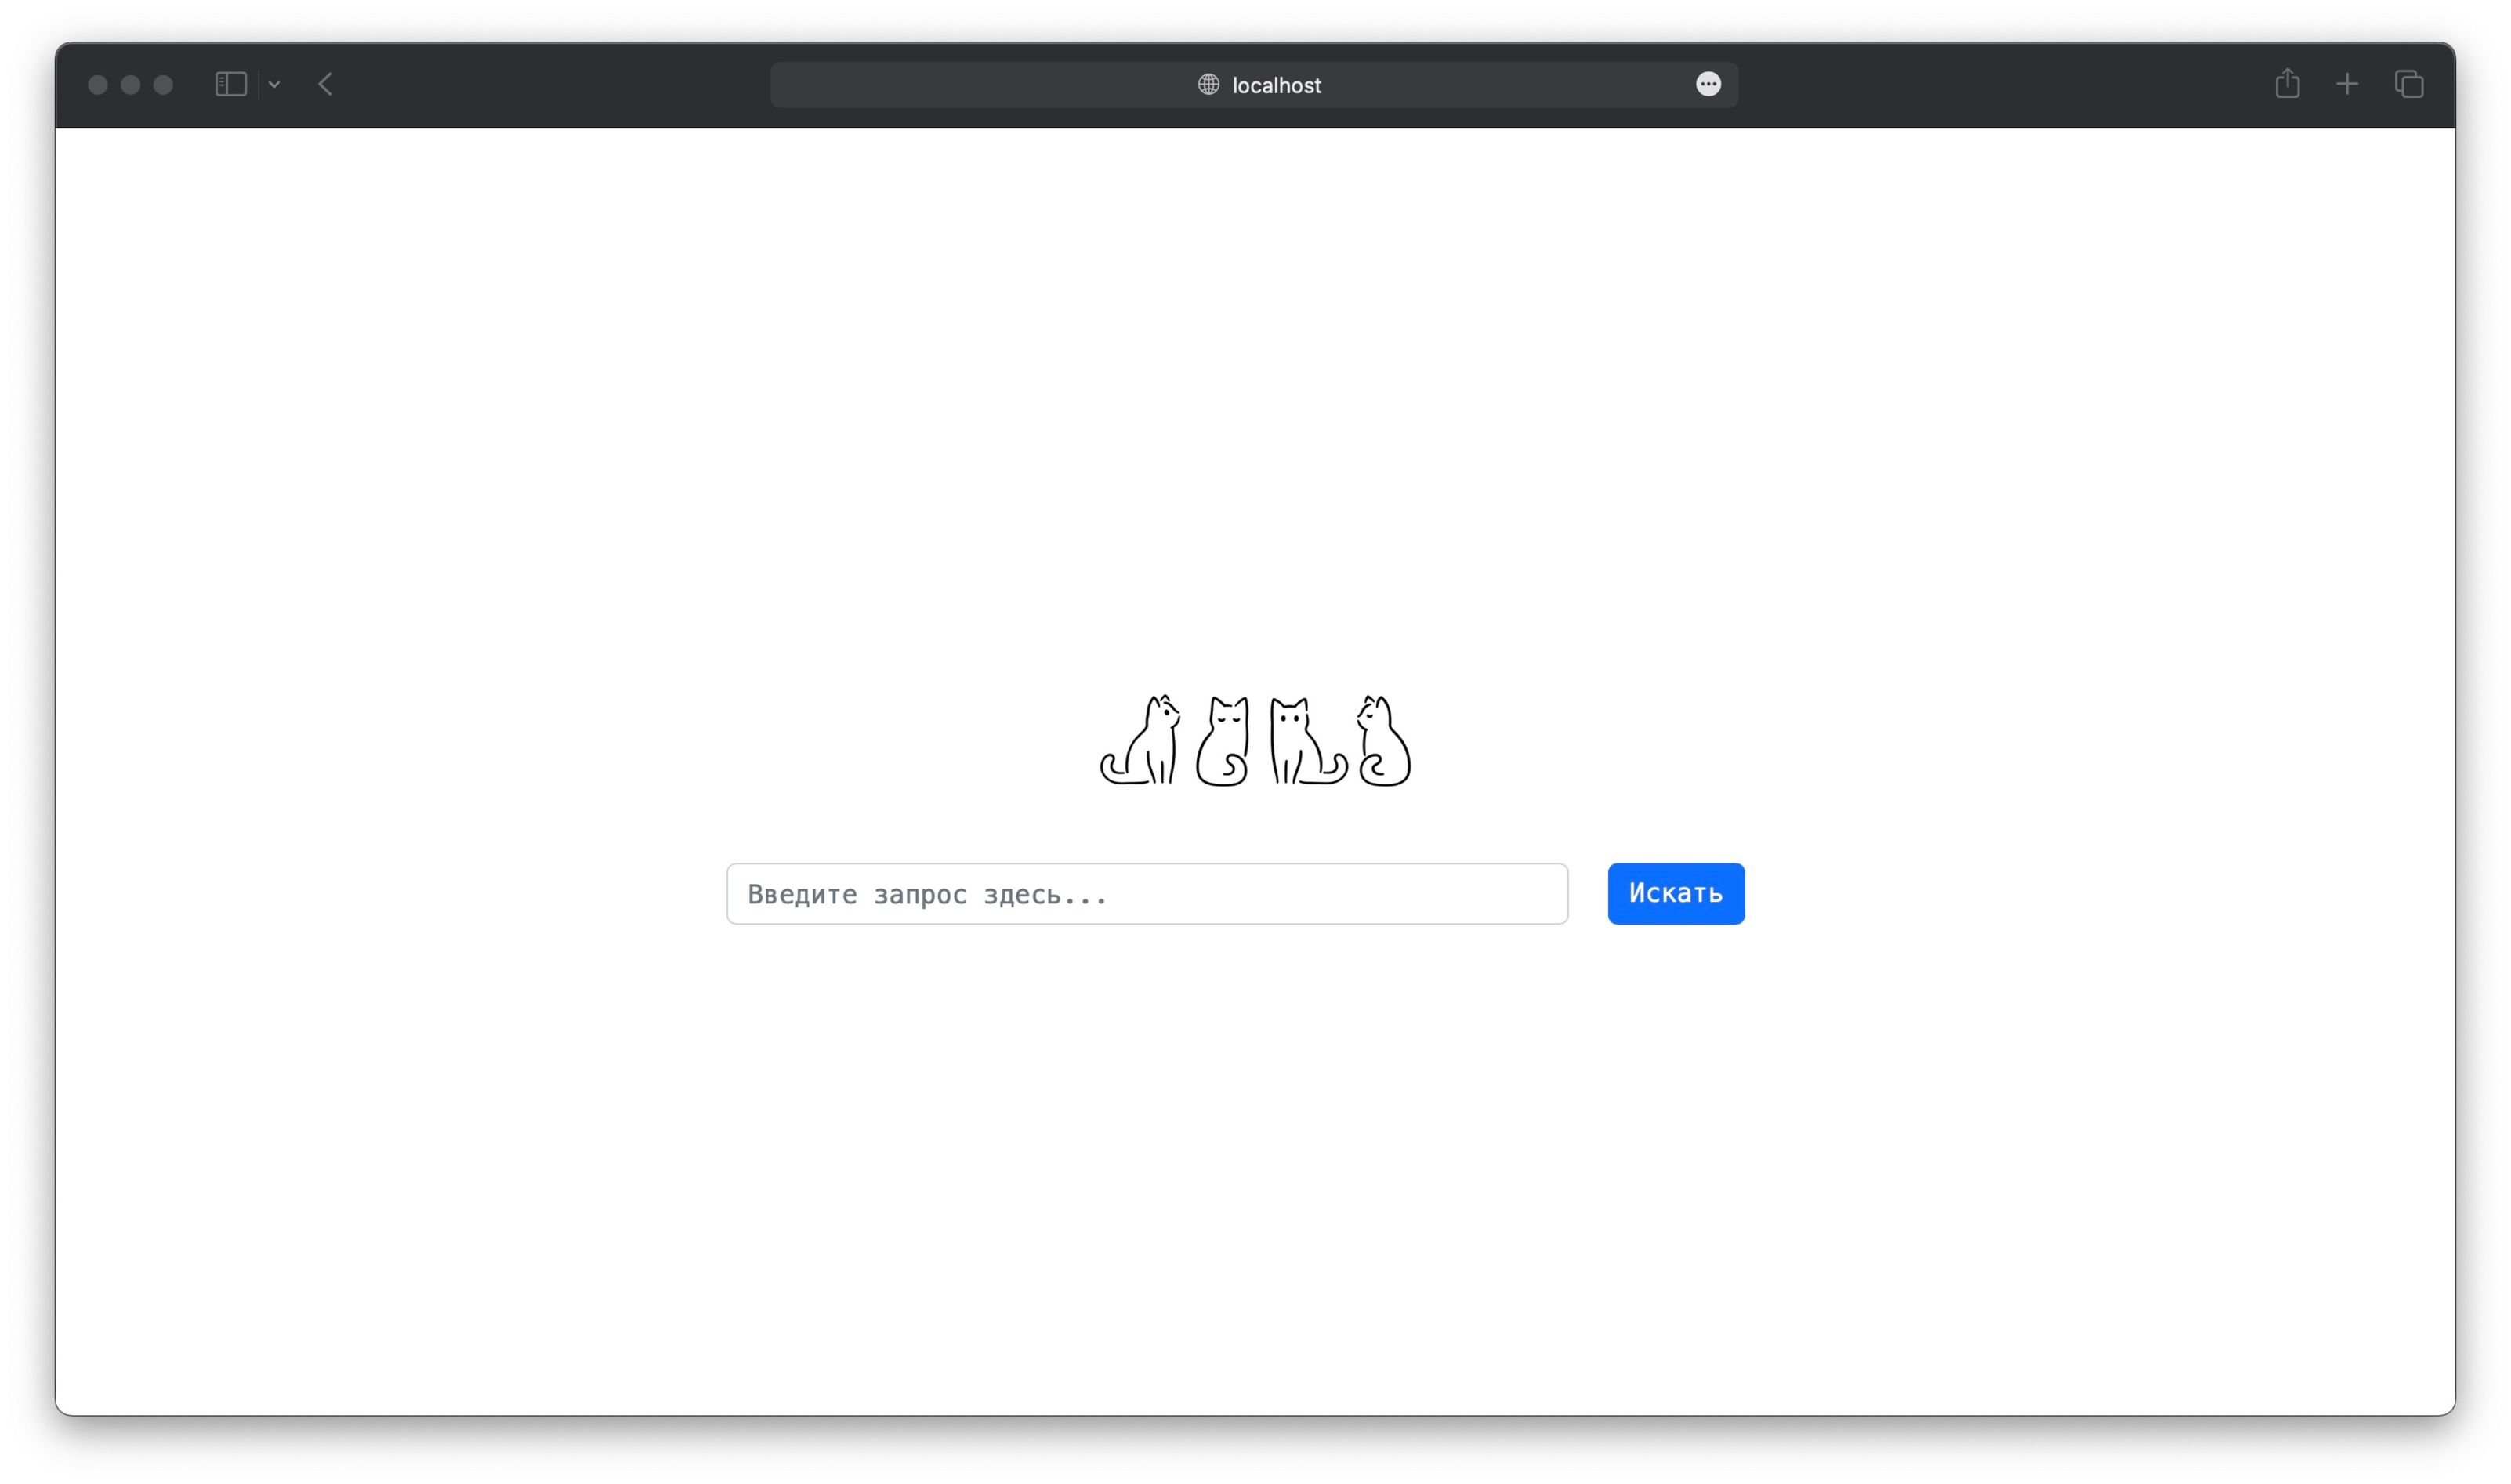
\includegraphics[width=0.9\linewidth]{int1.pdf}
    \caption{Интерфейс разработанного веб-сврвиса: домашняя страница}
    \label{img:int1}
\end{figure}

\begin{figure}[h!]
    \centering
    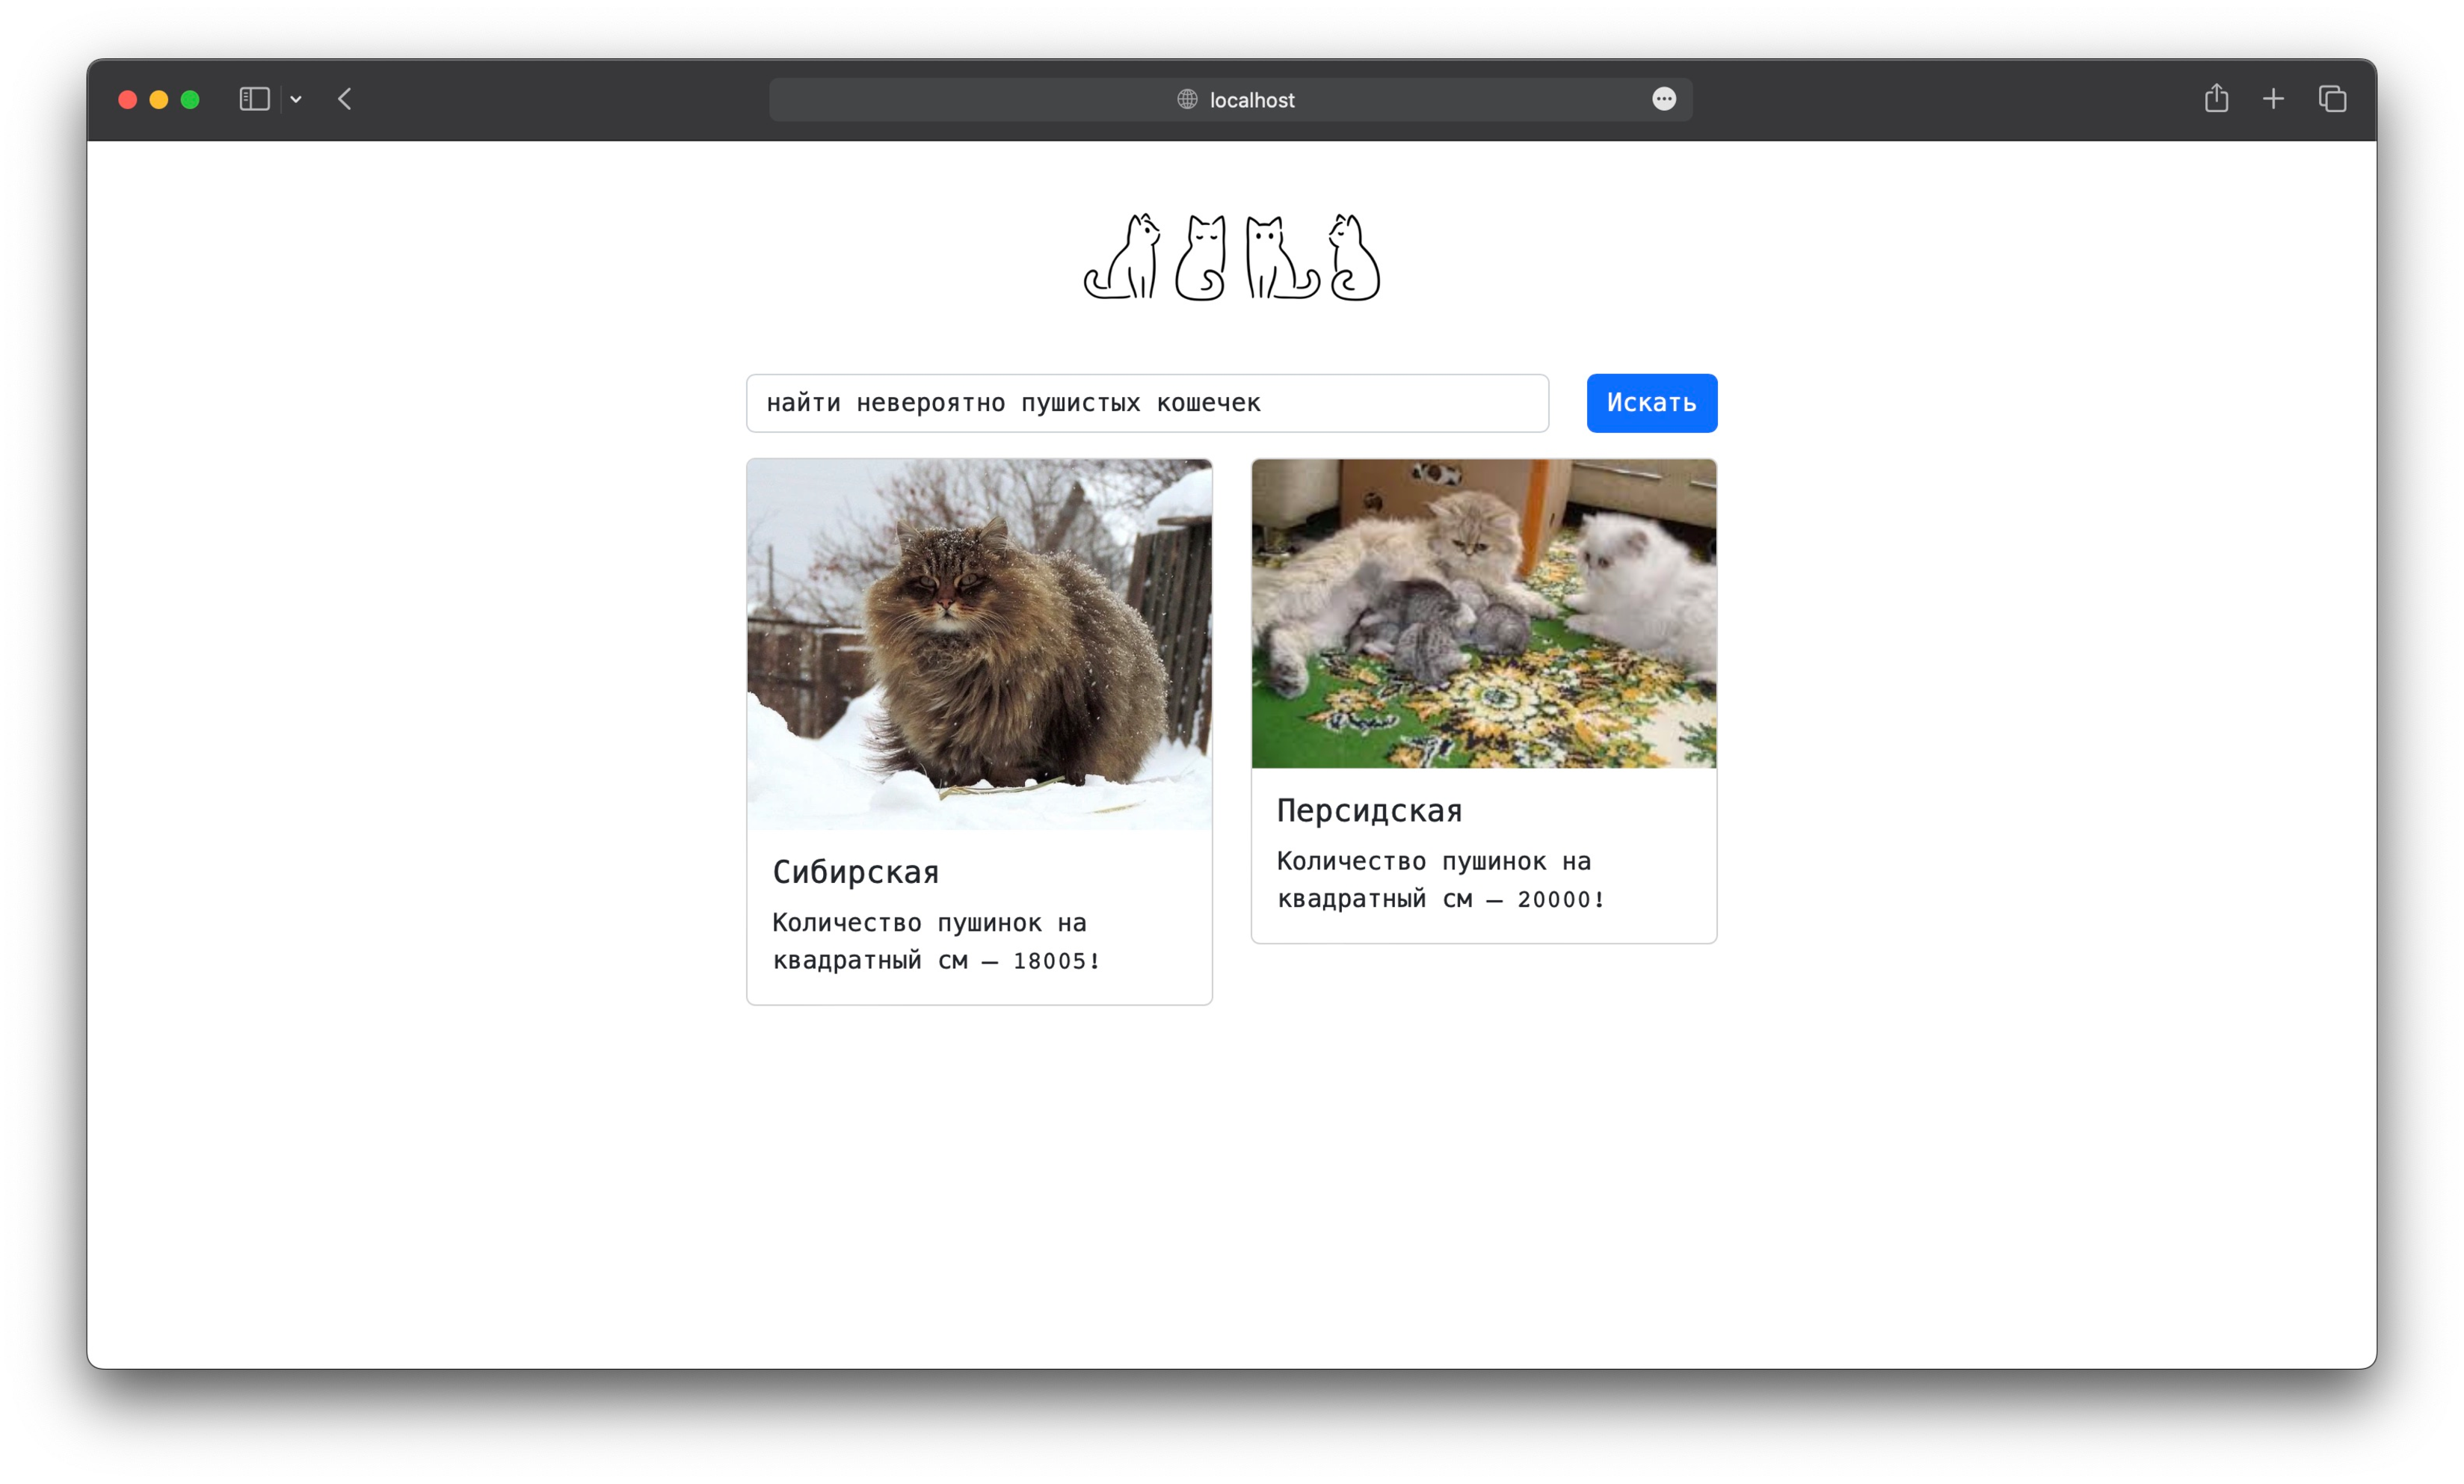
\includegraphics[width=0.9\linewidth]{int2.pdf}
    \caption{Интерфейс разработанного веб-сврвиса: страница поиска}
    \label{img:int2}
\end{figure}

\newpage